\documentclass[a4paper,12pt]{article}
\usepackage{amsfonts}
\usepackage{amssymb}
\usepackage{latexsym}
\usepackage{amsmath}
\usepackage{amsthm}
\usepackage{graphicx}
\usepackage{indentfirst}
\usepackage[polish]{babel}
\usepackage[T1]{fontenc}
\usepackage[utf8]{inputenc} % tu może być konieczne zastąpienie "cp1250" przez np. "utf8"
\usepackage{setspace}
\usepackage{array}
\usepackage{multirow}
\usepackage{geometry}
\usepackage{float}
\usepackage{wrapfig}
\geometry{hdivide={2cm,*,2cm}}
\geometry{vdivide={2cm,*,2cm}}
\usepackage{titlesec}
\titlespacing{\section}{0ex}{1ex}{1ex} % zmniejszenie odstępów przed i po tytule rozdziału...
\titleformat*{\section}{\sf\large\bfseries} % i zmiana kroju czcionki
\titlespacing{\subsection}{0ex}{0.75ex}{0.75ex} % % j/w dla tytułów podrozdziałów
\titleformat*{\subsection}{\sf\bfseries}

% Zmniejszenie odstępów przed i za wzorami wystawionymi
\AtBeginDocument{
\addtolength{\abovedisplayskip}{-1ex}
\addtolength{\abovedisplayshortskip}{-1ex}
\addtolength{\belowdisplayskip}{-1ex}
\addtolength{\belowdisplayshortskip}{-1ex}
}
% Kilka przydatnych definicji
\newcolumntype{C}[1]{>{\centering\arraybackslash}m{#1}}
\newcommand{\razy}{\hspace{-0.5ex}\times\hspace{-0.5ex}} % może się przydać


\begin{document}

\def\tablename{Tabela} % bez tej linii nazwą tabeli byłaby "Tablica"


\noindent
\textbf{Mikołaj Wałachowski, 320748, grupa J3, projekt 1, zadanie 6}


\section*{Wstęp} % section* oznacza rozdział bez numeru (zasadne przy braku spisu treści)
W celu otrzymania wyższego rzędu metody rozwiązywania równań różniczkowych zwyczajnych, stosuje się wzory $k$-krokowe \textit{Adamsa-Bashfortha}, zapewniające rząd $k$. Jednakże takie metody dalej opierają się na przewidywaniu kolejnych wartości funkcji na podstawie poprzednich $s$ węzłów. Takie podejście skutkuje istotną utratą dokładności przy równaniach źle uwarunkowanych numerycznie. Z tego też powodu stosuje się wzory \textit{Adamsa-Moultona}, które zwiększają precyzję omawianych metod, przeprowadzając w każdym kroku dodatkowe obliczenia, należy jednak pamiętać, że zastosowanie tych wzorów nie zwiększa rzędu metody. Ten raport ma na celu eksperymentalne zweryfikowanie własności numerycznych wyżej wspomnianych metod.

\section*{Opis metody Adamsa-Bashfortha-Moultona 2-go rzędu}
Załóżmy, że mamy równanie różniczkowe $m$-tego rzędu dane wzorem
\begin{align}
y^{(m)} = f(x,y,y',y'',...,y^{(m-1)})
\end{align}
Zdefiniujmy na podstawie $(1)$
\begin{align*}
Y \equiv \begin{bmatrix} 
        y_1\\
        y_2\\
        y_3\\
        \vdots\\
        y_{m+1}
        \end{bmatrix}
        =
        \begin{bmatrix}
        x\\
        y\\
        y'\\
        \vdots\\
        y^{(m-1)}
        \end{bmatrix}
        ,\qquad F \equiv F(Y) = \begin{bmatrix} 
        1\\
        y_3\\
        y_4\\
        \vdots\\
        f(x,y_1,y_2,...,y_{m+1})
        \end{bmatrix}.
\end{align*}
Wtedy dla przedziału $[a,b]$ oraz kroku całkowania $h$, pierwsze przybliżenie $Y_1$ znajdujemy przy pomocy zmodyfikowanej metody Eulera danej wzorem
\begin{align*}
    Y_1 = Y_0 + hF(Y_0 + \frac{h}{2}F(Y_0)).
\end{align*}
Dla każdego kolejnego $i$-węzła liczymy teraz kolejno predyktor dany wzorem \textit{Adamsa-Bashfortha}
\begin{align}
    Y_i = Y_{i-1} + \frac{3}{2}hF(Y_{i-1}) - \frac{1}{2}hF(Y_{i-2})
\end{align}
oraz korektor dany wzorem \textit{Adamsa-Moultona}
\begin{align}
    Y_i = Y_{i-1} + \frac{h}{2}(F(Y_{i}) + F(Y_{i-1})),
\end{align}
gdzie $Y_i$, użyte po prawej stronie równania, to predyktor wyliczony wzorem \textit{Adamsa-Bashfortha}. Każdy z wyżej przedstawionych wzorów jest 2-go rzędu więc metoda \textit{Adamsa-Bashfortha-Moultona} również będzie 2-go rzędu. 
\section*{Eksperymenty numeryczne}
Zgodnie z własnościami metod 2-go rzędu dla $e^{(h)}$ - maksymalnego błędu globalnego przy kroku $h$, powinno zostać spełnione $e^{(h)} = \mathcal{O}(h^2)$. Oznacza to że dla odpowiednio małego kroku całkowania powinniśmy otrzymać stosunek błędów - $d$, taki że
\begin{align}
d \equiv \frac{e^{(h_{i-1})}}{e^{(h_{i})}} \approx \left(\frac{h_{i-1}}{h_i}\right)^2.
\end{align}
Sprawdźmy teraz powyższą tezę dla równania $\cos(x)y' + \sin(x)y = 1$, dla warunku początkowego $y(0) = 1$, na przedziale $[0,1]$. W tym celu będziemy porównywać maksymalne błędy globalne a także ich stosunek $d$, dla kolejnych kroków całkowania, zmniejszając go za każdym razem czterokrotnie. W wynikach zestawionych w tabeli 1 widać, że dla odpowiednio małego kroku całkowania stosunek błędów - $d$ zbliża się do $16$, co potwierdza zależność $(4)$. Inne przeprowadzone testy poprawności, dla różnych uwarunkowań, również potwierdzają ten wynik.

\begin{wraptable}{r}{4cm}
\centering
\caption{}
\vspace{1mm}
\begin{tabular}{|l|l|l|}
\hline
\multicolumn{1}{|c|}{$h$}      & \multicolumn{1}{c|}{$e^{(h)}$} & \multicolumn{1}{c|}{$d$}   \\ \hline
\multicolumn{1}{|c|}{0.100000} & \multicolumn{1}{c|}{2.21e-04}  & \multicolumn{1}{c|}{}  \\
\multicolumn{1}{|c|}{0.025000} & \multicolumn{1}{c|}{1.64e-05}  & \multicolumn{1}{c|}{13.51} \\
0.006250                       & 1.08e-06                       & 15.21                      \\
0.001563                       & 6.83e-08                       & 15.79                      \\
0.000391                       & 4.28e-09                       & 15.95                      \\ \hline
\end{tabular}

\caption{}
\vspace{1mm}
\begin{tabular}{|l|l|l|}
\hline
\multicolumn{1}{|c|}{$h$}      & \multicolumn{1}{c|}{$e^{(h)}$} & \multicolumn{1}{c|}{$d$}   \\ \hline
\multicolumn{1}{|c|}{0.100000} & \multicolumn{1}{c|}{1.27e-03}  & \multicolumn{1}{c|}{}  \\
\multicolumn{1}{|c|}{0.025000} & \multicolumn{1}{c|}{8.56e-05}  & \multicolumn{1}{c|}{14.83} \\
0.006250                       & 5.45e-06                       & 15.70                      \\
0.001563                       & 3.42e-07                       & 15.93                      \\
0.000391                       & 2.14e-08                       & 15.98                      \\ \hline
\end{tabular}

\end{wraptable}
Przeprowadźmy teraz analogiczny eksperyment, tylko że tym razem wyłączony zostanie korektor. W tym przypadku cała procedura będzie wyglądała tak samo z tą tylko różnicą, że nie będziemy korzystać ze wzoru $(3)$, oznacza to że wykonujemy teraz dwukrokową metodę \textit{Adamsa-Bashfortha}, określoną wzorem $(2)$. Zauważmy, że z wyników eksperymentu przedstawionych w tabeli 2 wynika, że wyłączenie korektora nie skutkuje zmniejszeniem rzędu metody. Pozostaje więc pytanie jaki jest cel używania wzoru \textit{Adamsa-Moultona}, skoro wymaga on dodatkowych obliczeń, a wcale nie zwiększa rzędu metody.\\
Zauważmy, że jawne wzory wielokrokowe opierają się na przewidywaniu wartości funkcji, jedynie na podstawie jej wartości (a także jej pochodnych) w poprzednich węzłach. Taka procedura bywa wadliwa, gdy pojawiają się pewne niestabilności (na przykład, gdy mamy duży krok całkowania, albo zadane równanie jest źle uwarunkowane numerycznie). Aby rozważyć takie przypadki oznaczmy
\begin{align*}
    \epsilon \equiv \max\left| \frac{Y_c - Y_p}{Y_c} \right|,
\end{align*}
gdzie $Y_p$ i $Y_c$, to wektory wartości funkcji policzone odpowiednio wzorami predyktor oraz predyktor-korektor. Wartość $\epsilon$ będzie wskazywała na to, jak duży wpływ na precyzję metody miało zastosowanie wzoru korektor. Rozpatrzmy teraz zależność $\epsilon$ od kroku całkowania dla następujących równań różniczkowych przybliżanych na przedziale $[0,1]$.
\begin{table}[H]
\begin{tabular}{|cc|}
\hline
$y^{(IV)} + 4y = 0$      & $y(0) = 100, y'(0) = 0, y''(0) = 0, y'''(0) = 0$ \\ \hline
$cos(x)y' + sin(x)y = 1$ & $y(0) = 1$                                       \\ \hline
$y^{(IV)} - y = x^2$     & $y(0) = 1, y'(0) = 1, y''(0) = 1, y'''(0) = 1$   \\ \hline
\end{tabular}
\end{table}

%\begin{wrapfigure}{r}{0.75\textwidth}
\vspace{-20pt}
\begin{figure}[H]
    \hspace*{-1cm} 
    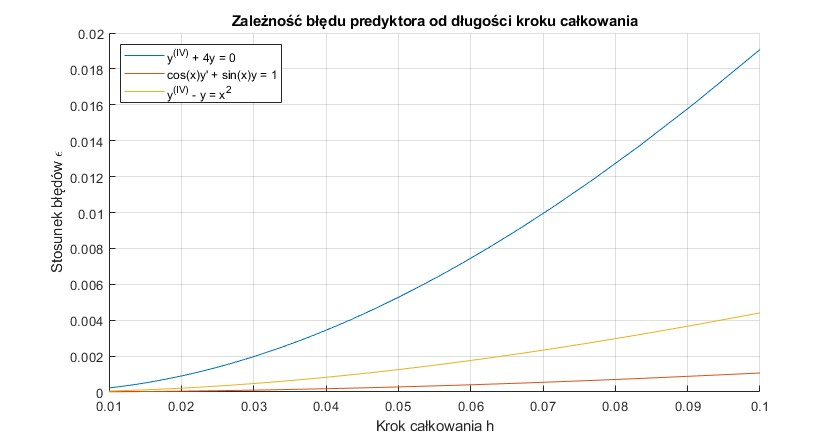
\includegraphics[width=1\textwidth]{predictor_error_graph.jpg}
\end{figure}

%\end{wrapfigure}
Zgodnie z przewidywaniami wraz ze wzrostem kroku całkowania zastosowanie wzoru korektor ma coraz większy wpływ na precyzję metody. Warto jednak zaznaczyć, że eksperyment został przeprowadzony na stosunkowo bezpiecznych numerycznie równaniach w zadanym regionie. Dla mniej stabilnych równań wartość $\epsilon$ mogłaby być znacznie większa.\\ 
Powyższe rozważania pokazują, że pomimo braku wpływu na szybkość zbieżności metody, stosowanie wzoru \textit{Adamsa-Moultona} zapewnia inne znaczące korzyści. W szczególności, gdy stosujemy małą liczbę iteracji lub zadane równanie jest źle uwarunkowane.
%\section*{Dodatek}
\end{document}
